\section{Workflows}
\label{150:sec:workflows}

ExaBounds is part of a larger set of tools that together can be used for performance and power analysis of future (exascale) computing systems. The set of tools encompasses IBM Platform-Independent Software Analysis~\cite{Anghel2016} for hardware-independent application profiling. The generates profiles serve as input for the workload extrapolation models of IBM Exascale Extrapolator~\cite{Mariani2016} or directly to IBM ExaBounds.

Figure~\ref{fig:150:workflow} shows the potential workflows of our tooling. The lower part of the figure shows the most basic workflow: IBM Platform-Independent Software Analysis is used to profile a single run of an application. The generated profile (in JSON format) is loaded in IBM ExaBounds and predictions are made for an architecture of for a set of architectures (design-space exploration).

\begin{figure}
 \centering
 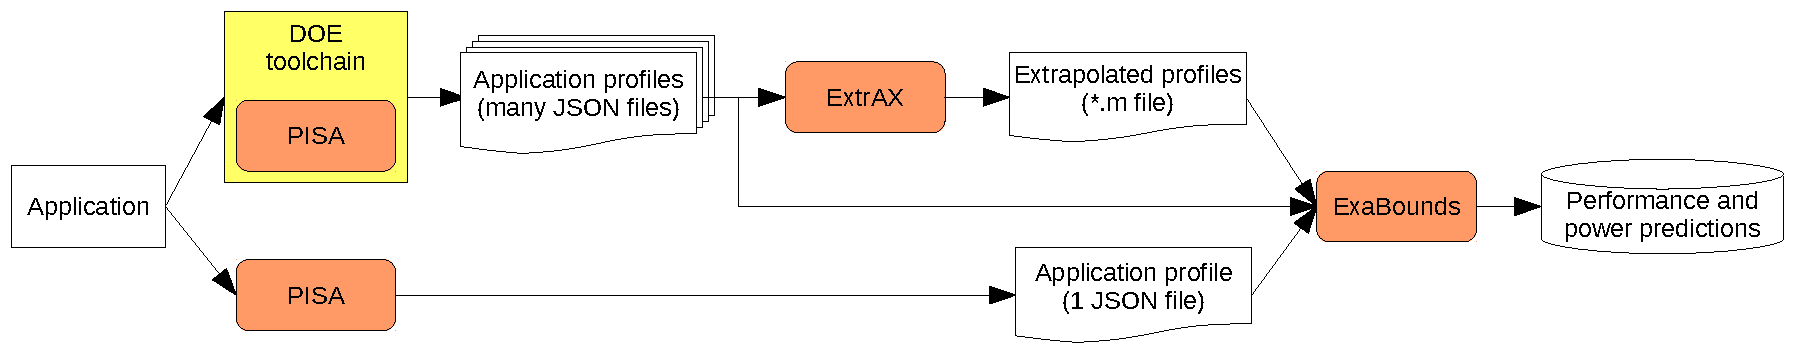
\includegraphics[width=\columnwidth]{img/workflow.pdf}
 \caption{Different workflows of our tool flow. IBM Platform-Independent Software Analysis is used to extract profiles of applications. Such profiles can be extrapolated to exascale using IBM Exascale Extrapolator. ExaBounds predicts the performance and power consumption of the application running on different architectures.}
 \label{fig:150:workflow}
\end{figure}

The top part of the figure shows a more complex workflow. Applications can behave differently for different workloads (both workload size or data content), or, for parallel applications, threads within an application may behave differently for different amounts of exploited parallelism. To capture this dynamism, a design of experiments (DOE) can be performed to sample the behavior of the application at different operating points. This will involve multiple runs of the profiler and will result in a set of JSON output files. These output files can subsequently be directly used in ExaBounds for performance and power predictions, but it is also possible to first use IBM Exascale Extrapolator to extrapolate the workload profiles to a point that isn't sampled (using machine learning). As an example, the application profiles can be exploited to an exascale-sized workload, a workload size that cannot be analyzed by IBM Platform-Independent Software Analysis directly due to constraints on the system which is used for profiling. IBM Exascale Extrapolator generates a Mathematica file containing the profiles of the application at the targed (scaled) operating points. This Mathematica file can be similarly read by IBM ExaBounds for predictions.

\section{Default architectures and algorithms}

\begin{minipage}[t]{0.05\textwidth}
~\\
\Huge !
\end{minipage}
\begin{minipage}[t]{0.94\textwidth}
IBM ExaBounds ships with a set of default loaded architectures and algorithms. The architectural properties aim to reflect their respective architectures as good as possible. Most properties are retrieved from public sources on the Internet. Some of the remaining properties cannot be found and are based on reasonable estimates. It is advised to carefully check default architectures and algorithms for correctness for real experiments.\end{minipage}
~\linebreak
